\chapter{Estratégias de negociação com o BVRP previsto}
\label{app:estrategias}

Este apêndice traduz em regras simples de negociação a relação entre o BVRP
previsto e os retornos futuros estudada nos
Capítulos~\ref{chap:retornos_linear} e~\ref{chap:retornos_nao_linear}. A
análise é exploratória. Nenhum dos dois capítulos encontra previsibilidade dos
retornos que resista às correções para o regressor gerado e para as
comparações múltiplas, e o apêndice não apresenta as regras a seguir como fonte
de retorno excedente. Elas mostram como o coeficiente negativo do
Capítulo~\ref{chap:retornos_linear} se traduz no desempenho de uma posição no
mercado à vista, antes e depois dos custos de transação.

% =========================================================
\section{Desenho}
\label{sec:estr-desenho}

\paragraph{Sinal.} O sinal principal é $\widehat{\text{BVRP}}_t$, a previsão
do Ridge em janela expansiva do Capítulo~\ref{chap:previsao_bvrp}, a mesma que
serve de regressor no Capítulo~\ref{chap:retornos_linear}; a previsão de $t$ só
usa informação disponível até $t$. Como teste de robustez, a mesma regra é
aplicada à proxy retrospectiva,
$\text{BVRP}^{\text{proxy}}_t = \text{VH}_{t-29:t} - \text{IV}_t$, também
conhecida em $t$.

\paragraph{Regra.} Em cada data, o limiar $q(t)$ é o quantil $q$ do sinal nas
observações até $t$, em janela expansiva, e o sinal é alto quando
$\widehat{\text{BVRP}}_t \ge q(t)$. A regra define a posição no fim de $t$ e a
aplica ao retorno simples de $t$ a $t+1$; nenhuma informação posterior a $t$
entra na decisão. O cálculo do limiar começa na 252ª previsão. Como as
previsões começam em 21/06/2023, a negociação com o Ridge vai de 27/02/2024 a
02/03/2026, 735 dias; a última data da amostra, 03/03/2026, fica de fora porque
o retorno seguinte cairia depois dela. Com um \textit{burn-in} de 126
previsões, como sensibilidade, a negociação começa em 24/10/2023 (861 dias). O
quantil de referência é o de 80\%; as tabelas reportam ao lado os de 60\%,
70\% e 90\%.

\paragraph{Direções.} Com o sinal alto, a regra comprada/neutra fica comprada
em uma unidade de Bitcoin, e a vendida/neutra, vendida em uma unidade; nos
outros dias, as duas ficam fora do mercado. A dissertação fixou as duas
direções antes de ver os resultados e as reporta juntas, para que a direção
não seja escolhida depois deles. Sem custos, o retorno diário da vendida é o da
comprada com o sinal trocado, e o índice de Sharpe também.

\paragraph{Custos.} Os custos são unilaterais, de 0, 10 e 30 pontos-base
(bps) por mudança de posição. Os 10 bps correspondem à taxa \textit{taker}
padrão da Binance no mercado à vista \citep{Binance2024fees}; os 30 bps são um
cenário mais oneroso, que deixa margem para \textit{spread} e execução
desfavoráveis.

\paragraph{Métricas.} As métricas são anualizadas com 365 dias, pois o mercado
funciona todos os dias. O índice de Sharpe \citep{sharpe1994sharpe} é a média
do retorno diário vezes 365 dividida pelo desvio-padrão diário vezes
$\sqrt{365}$, sem taxa livre de risco. O índice de Sortino
\citep{sortino1994performance} troca o desvio-padrão pelo desvio abaixo de um
retorno mínimo aceitável, aqui zero: $\sqrt{\text{média}(\min(r_t, 0)^2)}$,
calculado sobre todos os dias e anualizado da mesma forma. O
\textit{drawdown} máximo é a maior queda do valor acumulado em relação ao pico
anterior, a partir do valor inicial 1. A referência é o compra e manutenção do
Bitcoin nas mesmas datas, sem custo.

\paragraph{Regimes.} O regime de alta volatilidade é o da
Seção~\ref{sec:met-regimes}, $\text{VH}_{t-29:t} > 37{,}3\%$ a.a. Na análise
por regime, a regra só opera nos dias do regime e fica fora do mercado nos
demais; o compra e manutenção de cada regime é definido da mesma forma.

% =========================================================
\section{Resultados com o BVRP previsto}
\label{sec:estr-principal}

A Tabela~\ref{tab:estr-principal} e a Figura~\ref{fig:estr-principal}
apresentam as duas regras no quantil de 80\%. A comprada/neutra tem índice de
Sharpe de $-0{,}25$ sem custos, $-0{,}35$ com 10 bps e $-0{,}55$ com 30 bps.
Esse resultado é o que o Capítulo~\ref{chap:retornos_linear} antecipa: o coeficiente do
retorno futuro sobre o BVRP previsto é negativo em todos os horizontes ($-0{,}045$
em $h = 1$, com valor-$p$ de 0,043 no bootstrap, sem passar pelo limite de
Bonferroni). Um BVRP previsto alto antecede retornos menores, e a regra que
compra nesses dias perde.

\begin{table}[H]
\centering
\small
\caption{Estratégias com o BVRP previsto pelo Ridge (quantil 80\%, 27/02/2024 a 02/03/2026, 735 dias).}
\label{tab:estr-principal}
\resizebox{\textwidth}{!}{%
\begin{tabular}{llrrrrrrrr}
\toprule
Regra & Custo (bps) & Ret. anual (\%) & Vol. (\%) & Sharpe & Sortino & DD máx. (\%) & Giro (op./ano) & Operações & Tempo posic. (\%) \\
\midrule
Comprada/neutra & 0 & $-$9{,}3 & 25{,}5 & $-$0{,}25 & $-$0{,}36 & $-$28{,}2 & 24{,}8 & 50 & 41{,}0 \\
 & 10 & $-$11{,}5 & 25{,}5 & $-$0{,}35 & $-$0{,}50 & $-$29{,}3 & 24{,}8 & 50 & 41{,}0 \\
 & 30 & $-$15{,}8 & 25{,}6 & $-$0{,}55 & $-$0{,}77 & $-$31{,}4 & 24{,}8 & 50 & 41{,}0 \\
\midrule
Vendida/neutra & 0 & 3{,}3 & 25{,}5 & 0{,}25 & 0{,}36 & $-$39{,}9 & 24{,}8 & 50 & 41{,}0 \\
 & 10 & 0{,}7 & 25{,}5 & 0{,}16 & 0{,}22 & $-$41{,}5 & 24{,}8 & 50 & 41{,}0 \\
 & 30 & $-$4{,}2 & 25{,}6 & $-$0{,}04 & $-$0{,}05 & $-$44{,}5 & 24{,}8 & 50 & 41{,}0 \\
\midrule
Compra e manutenção & -- & 9{,}4 & 49{,}2 & 0{,}43 & 0{,}64 & $-$49{,}5 & -- & -- & 100{,}0 \\
\bottomrule
\end{tabular}}
\par\smallskip
\parbox{0.95\linewidth}{\footnotesize\textit{Nota}: Posição definida com informação até o fim de $t$ e aplicada ao retorno simples de $t$ a $t+1$; limiar no quantil $q$ do sinal em janela expansiva (observações até $t$). Custos unilaterais sobre $|\Delta \text{posição}|$. Sharpe: média $\times$ 365 / (desvio-padrão $\times \sqrt{365}$), sem taxa livre de risco; Sortino: média $\times$ 365 / ($\sqrt{\text{média}(\min(r_t, 0)^2)} \times \sqrt{365}$), com todos os dias. DD máx.: drawdown máximo a partir do valor inicial 1. Compra e manutenção nas mesmas datas, sem custo. Sem custos, o retorno diário da regra vendida/neutra é o da comprada/neutra com o sinal trocado. Burn-in de 252 previsões do Ridge.}
\end{table}


Sharpe e Sortino negativos na regra comprada indicam que a posição lucrativa
seria a vendida, e a regra vendida/neutra verifica isso diretamente: Sharpe de
0,25 sem custos e de 0,16 com 10 bps, e Sortino de 0,36 sem custos. Com 30 bps,
o Sharpe cai para $-0{,}04$. O ganho da vendida tem a mesma fragilidade do
coeficiente do Capítulo~\ref{chap:retornos_linear}, que não é significante
depois das correções, e a Figura~\ref{fig:estr-principal} mostra que ele se
concentra no fim da amostra: a vendida só termina acima do valor inicial com a
queda do Bitcoin em janeiro e fevereiro de 2026.

Nenhuma das duas regras supera o compra e manutenção no mesmo período, com
Sharpe de 0,43 e Sortino de 0,64. O que as regras oferecem é um
\textit{drawdown} máximo menor: $-28{,}2\%$ na comprada e $-39{,}9\%$ na
vendida, contra $-49{,}5\%$ no compra e manutenção, cujo pior momento é a queda
de fevereiro de 2026. A redução vem da menor exposição --- as regras ficam
posicionadas em 41\% dos dias, com volatilidade anual de 25,5\%, contra 49,2\%
do compra e manutenção ---, e não de informação sobre a direção dos retornos: a
comprada reduz o \textit{drawdown} com Sharpe negativo.

\IfFileExists{figs/estrategias/fig_principal.png}{
\begin{figure}[H]
    \centering
    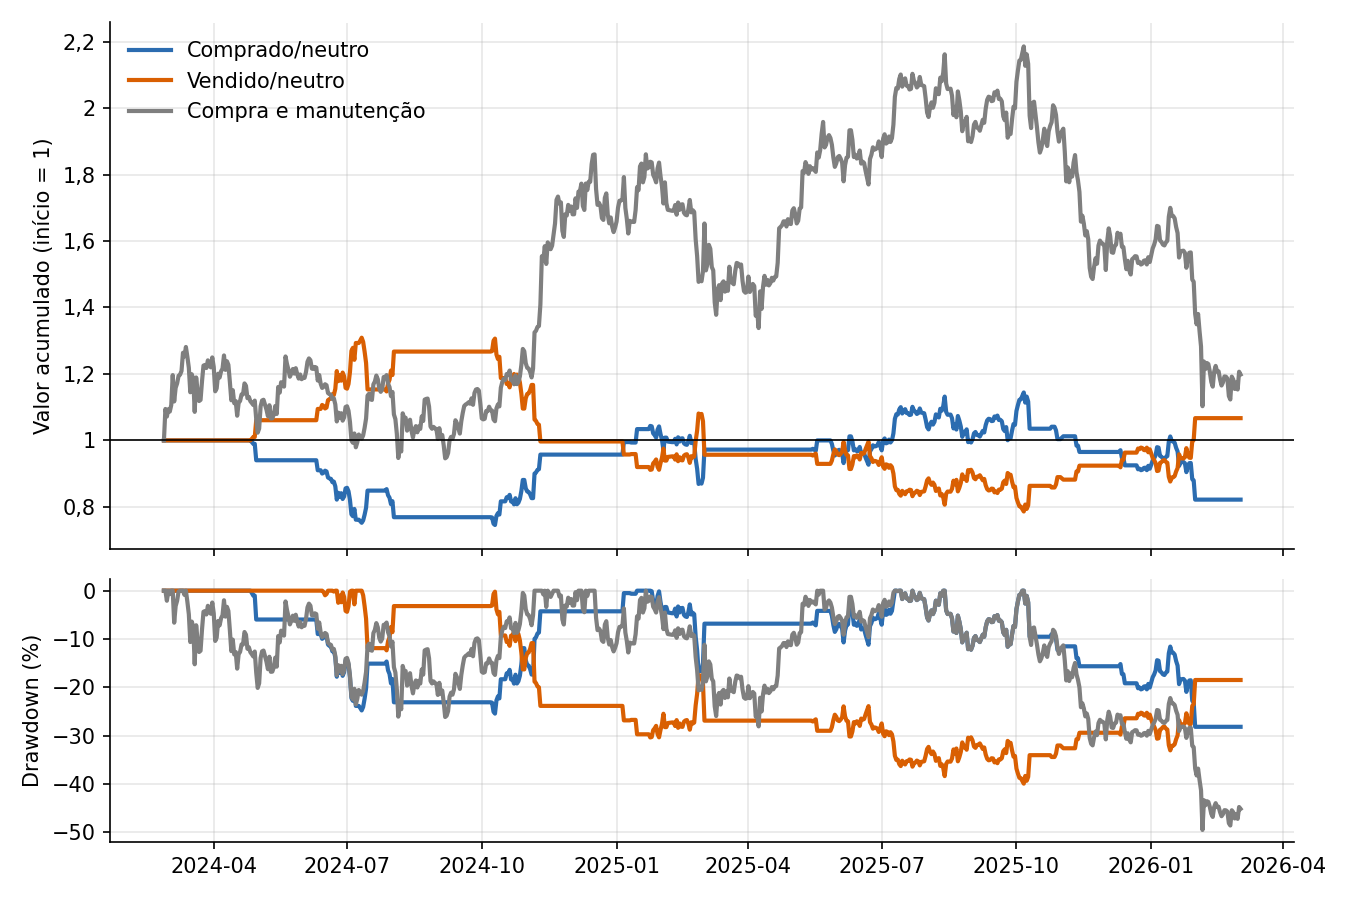
\includegraphics[width=0.9\linewidth]{figs/estrategias/fig_principal.png}
    \caption{Valor acumulado (painel superior) e \textit{drawdown} (painel inferior) das regras comprada/neutra e vendida/neutra com o BVRP previsto pelo Ridge (quantil 80\%, sem custos) e do compra e manutenção, de 27/02/2024 a 02/03/2026.}
    \label{fig:estr-principal}
\end{figure}
}{}

% =========================================================
\section{Quantis}
\label{sec:estr-quantis}

A Tabela~\ref{tab:estr-quantis} e a Figura~\ref{fig:estr-quantis} repetem as
duas regras nos quantis de 60\% a 90\%. A comprada tem Sharpe negativo em todos
os quantis e custos, de $-0{,}14$ a $-0{,}39$ sem custos. A vendida tem Sharpe
positivo sem custos em todos eles (0,14 no q60, 0,34 no q70, 0,25 no q80 e 0,39
no q90); com 30 bps, só o q70 e o q90 continuam positivos (0,09 e 0,05).
Nenhuma combinação alcança o Sharpe de 0,43 do compra e manutenção.

\begin{table}[H]
\centering
\small
\caption{Estratégias com o BVRP previsto pelo Ridge, por quantil (27/02/2024 a 02/03/2026).}
\label{tab:estr-quantis}
\resizebox{\textwidth}{!}{%
\begin{tabular}{llrrrrrrr}
\toprule
Regra & Quantil & Sharpe (0) & Sharpe (10) & Sharpe (30) & Sortino & DD máx. (\%) & Giro (op./ano) & Tempo posic. (\%) \\
\midrule
Comprada/neutra & q60 & $-$0{,}14 & $-$0{,}22 & $-$0{,}40 & $-$0{,}20 & $-$46{,}6 & 27{,}8 & 59{,}3 \\
 & q70 & $-$0{,}34 & $-$0{,}42 & $-$0{,}59 & $-$0{,}48 & $-$40{,}6 & 24{,}8 & 50{,}7 \\
 & q80 & $-$0{,}25 & $-$0{,}35 & $-$0{,}55 & $-$0{,}36 & $-$28{,}2 & 24{,}8 & 41{,}0 \\
 & q90 & $-$0{,}39 & $-$0{,}50 & $-$0{,}72 & $-$0{,}53 & $-$23{,}9 & 19{,}9 & 26{,}5 \\
\midrule
Vendida/neutra & q60 & 0{,}14 & 0{,}05 & $-$0{,}12 & 0{,}19 & $-$58{,}0 & 27{,}8 & 59{,}3 \\
 & q70 & 0{,}34 & 0{,}25 & 0{,}09 & 0{,}48 & $-$49{,}0 & 24{,}8 & 50{,}7 \\
 & q80 & 0{,}25 & 0{,}16 & $-$0{,}04 & 0{,}36 & $-$39{,}9 & 24{,}8 & 41{,}0 \\
 & q90 & 0{,}39 & 0{,}28 & 0{,}05 & 0{,}57 & $-$19{,}8 & 19{,}9 & 26{,}5 \\
\midrule
Compra e manutenção & -- & 0{,}43 & -- & -- & 0{,}64 & $-$49{,}5 & -- & 100{,}0 \\
\bottomrule
\end{tabular}}
\par\smallskip
\parbox{0.95\linewidth}{\footnotesize\textit{Nota}: Posição definida com informação até o fim de $t$ e aplicada ao retorno simples de $t$ a $t+1$; limiar no quantil $q$ do sinal em janela expansiva (observações até $t$). Custos unilaterais sobre $|\Delta \text{posição}|$. Sharpe: média $\times$ 365 / (desvio-padrão $\times \sqrt{365}$), sem taxa livre de risco; Sortino: média $\times$ 365 / ($\sqrt{\text{média}(\min(r_t, 0)^2)} \times \sqrt{365}$), com todos os dias. DD máx.: drawdown máximo a partir do valor inicial 1. Compra e manutenção nas mesmas datas, sem custo. Sem custos, o retorno diário da regra vendida/neutra é o da comprada/neutra com o sinal trocado. Entre parênteses, o custo em bps; Sortino, drawdown, giro e tempo sem custos.}
\end{table}


Na comprada, o \textit{drawdown} diminui com o quantil, de $-46{,}6\%$ no q60 a
$-23{,}9\%$ no q90, junto com o tempo posicionado (de 59,3\% a 26,5\% dos dias),
o que confirma que a proteção vem da exposição menor. Na vendida, a relação é a
mesma, mas o q60 tem \textit{drawdown} de $-58{,}0\%$, maior que o do compra e
manutenção.

\IfFileExists{figs/estrategias/fig_quantis.png}{
\begin{figure}[H]
    \centering
    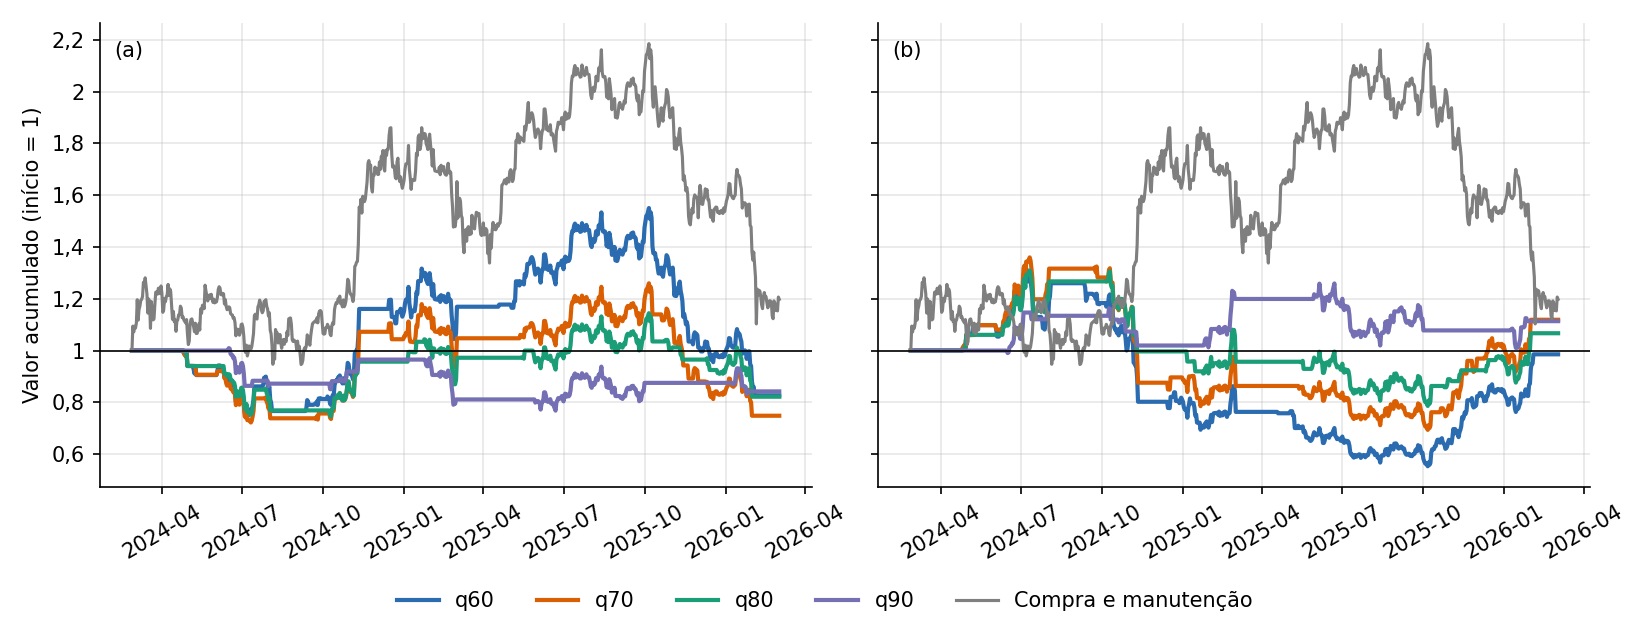
\includegraphics[width=\linewidth]{figs/estrategias/fig_quantis.png}
    \caption{Valor acumulado das regras com o BVRP previsto pelo Ridge, por quantil, sem custos: (a) comprada/neutra e (b) vendida/neutra, com o compra e manutenção como referência, de 27/02/2024 a 02/03/2026.}
    \label{fig:estr-quantis}
\end{figure}
}{}

% =========================================================
\section{Testes de robustez}
\label{sec:estr-robustez}

A Tabela~\ref{tab:estr-robustez} reúne três testes de robustez no quantil de
80\%. Com \textit{burn-in} de 126 previsões, o quadro é o mesmo: Sharpe de
$-0{,}23$ na comprada e de 0,23 na vendida ($-0{,}03$ com 30 bps). Os quatro
meses a mais, de outubro de 2023 a fevereiro de 2024, são de forte alta do
Bitcoin, e o Sharpe do compra e manutenção sobe para 0,85.

\begin{table}[H]
\centering
\small
\caption{Testes de robustez: burn-in e proxy retrospectiva (quantil 80\%).}
\label{tab:estr-robustez}
\resizebox{\textwidth}{!}{%
\begin{tabular}{lllrrrrrr}
\toprule
Sinal & Período & Dias & Regra & Sharpe (0) & Sharpe (10) & Sharpe (30) & DD máx. (\%) & Tempo posic. (\%) \\
\midrule
$\widehat{\text{BVRP}}_t$ (Ridge), burn-in de 252 & 27/02/2024--02/03/2026 & 735 & Comprada/neutra & $-$0{,}25 & $-$0{,}35 & $-$0{,}55 & $-$28{,}2 & 41{,}0 \\
 &  &  & Vendida/neutra & 0{,}25 & 0{,}16 & $-$0{,}04 & $-$39{,}9 & 41{,}0 \\
 &  &  & Compra e manutenção & 0{,}43 & -- & -- & $-$49{,}5 & 100{,}0 \\
\midrule
$\widehat{\text{BVRP}}_t$ (Ridge), burn-in de 126 & 24/10/2023--02/03/2026 & 861 & Comprada/neutra & $-$0{,}23 & $-$0{,}32 & $-$0{,}50 & $-$28{,}2 & 35{,}0 \\
 &  &  & Vendida/neutra & 0{,}23 & 0{,}15 & $-$0{,}03 & $-$39{,}9 & 35{,}0 \\
 &  &  & Compra e manutenção & 0{,}85 & -- & -- & $-$49{,}5 & 100{,}0 \\
\midrule
$\text{BVRP}^{\text{proxy}}_t$, amostra completa & 30/11/2021--02/03/2026 & 1.554 & Comprada/neutra & 0{,}13 & 0{,}03 & $-$0{,}17 & $-$36{,}4 & 26{,}3 \\
 &  &  & Vendida/neutra & $-$0{,}13 & $-$0{,}23 & $-$0{,}44 & $-$49{,}0 & 26{,}3 \\
 &  &  & Compra e manutenção & 0{,}34 & -- & -- & $-$72{,}4 & 100{,}0 \\
\midrule
$\text{BVRP}^{\text{proxy}}_t$, datas do Ridge & 27/02/2024--02/03/2026 & 735 & Comprada/neutra & 0{,}02 & $-$0{,}08 & $-$0{,}26 & $-$27{,}3 & 25{,}2 \\
 &  &  & Vendida/neutra & $-$0{,}02 & $-$0{,}11 & $-$0{,}30 & $-$33{,}3 & 25{,}2 \\
 &  &  & Compra e manutenção & 0{,}43 & -- & -- & $-$49{,}5 & 100{,}0 \\
\bottomrule
\end{tabular}}
\par\smallskip
\parbox{0.95\linewidth}{\footnotesize\textit{Nota}: Posição definida com informação até o fim de $t$ e aplicada ao retorno simples de $t$ a $t+1$; limiar no quantil $q$ do sinal em janela expansiva (observações até $t$). Custos unilaterais sobre $|\Delta \text{posição}|$. Sharpe: média $\times$ 365 / (desvio-padrão $\times \sqrt{365}$), sem taxa livre de risco; Sortino: média $\times$ 365 / ($\sqrt{\text{média}(\min(r_t, 0)^2)} \times \sqrt{365}$), com todos os dias. DD máx.: drawdown máximo a partir do valor inicial 1. Compra e manutenção nas mesmas datas, sem custo. Sem custos, o retorno diário da regra vendida/neutra é o da comprada/neutra com o sinal trocado. $\text{BVRP}^{\text{proxy}}_t = \text{VH}_{t-29:t} - \text{IV}_t$, conhecida em $t$. Nas datas do Ridge, o limiar da proxy usa todo o histórico dela desde 2021.}
\end{table}


Com a proxy na amostra completa (1.554 dias, de 30/11/2021 a 02/03/2026), a
direção se inverte: a comprada tem Sharpe de 0,13 sem custos, 0,03 com 10 bps e
$-0{,}17$ com 30 bps, e a vendida, $-0{,}13$. O ganho é pequeno, fica abaixo do
Sharpe de 0,34 do compra e manutenção e desaparece com custos; o que se mantém
é o \textit{drawdown} menor ($-36{,}4\%$ contra $-72{,}4\%$), com a regra
posicionada em 26\% dos dias (Figura~\ref{fig:estr-proxy}).

Para separar o efeito do sinal do efeito do período, o apêndice avalia a proxy
também nas mesmas 735 datas do Ridge, com o limiar calculado sobre todo o histórico
dela desde 2021. Nessas datas, a comprada com a proxy tem Sharpe de 0,02,
contra $-0{,}25$ com o Ridge, e o compra e manutenção é o mesmo (0,43). A
diferença entre as duas regras vem do sinal, e não do período.

\IfFileExists{figs/estrategias/fig_proxy.png}{
\begin{figure}[H]
    \centering
    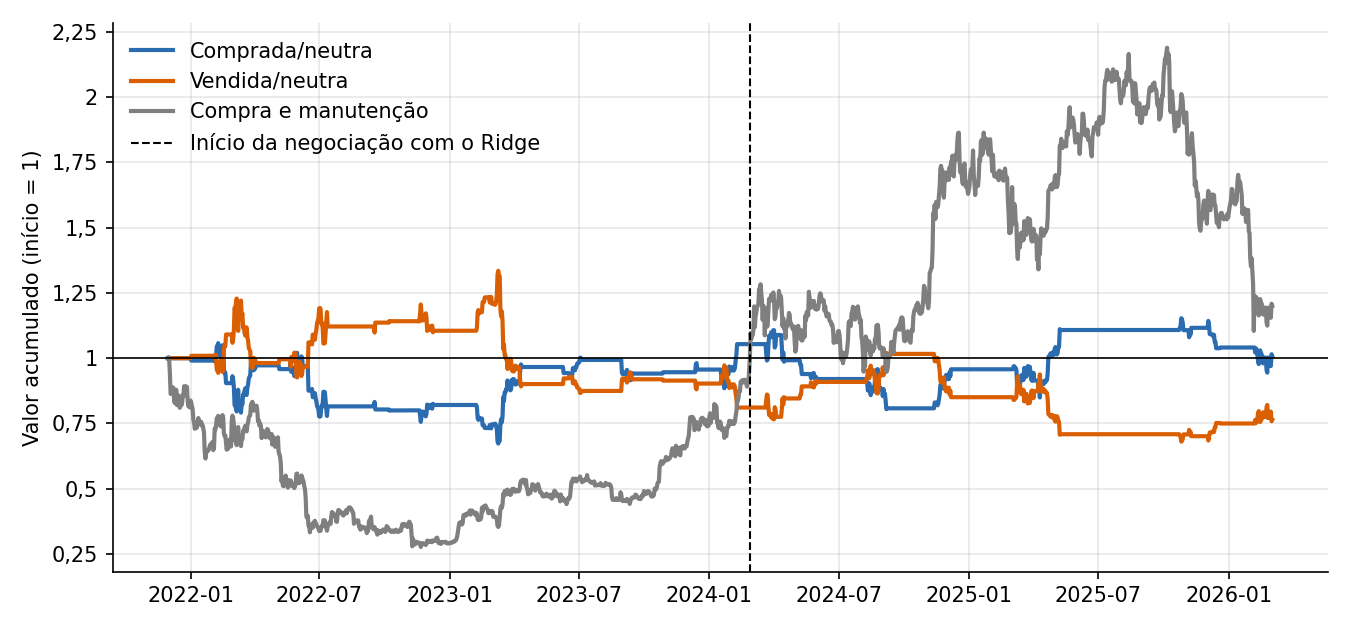
\includegraphics[width=0.9\linewidth]{figs/estrategias/fig_proxy.png}
    \caption{Valor acumulado das regras com $\text{BVRP}^{\text{proxy}}_t$ (quantil 80\%, sem custos) e do compra e manutenção, de 30/11/2021 a 02/03/2026. A linha tracejada marca o início da negociação com o BVRP previsto pelo Ridge (27/02/2024).}
    \label{fig:estr-proxy}
\end{figure}
}{}

% =========================================================
\section{Regimes de volatilidade}
\label{sec:estr-regimes}

A Tabela~\ref{tab:estr-regimes} aplica as regras em cada regime. Os períodos
diferem: com o Ridge, a análise cobre os mesmos 735 dias de negociação, de
27/02/2024 a 02/03/2026; com a proxy, começa em 21/06/2023, a primeira data das
previsões do Capítulo~\ref{chap:previsao_bvrp}, posterior à janela em que o
corte de $37{,}3\%$ a.a. foi estimado (986 dias).

\begin{table}[H]
\centering
\small
\caption{Estratégias por regime de volatilidade (quantil 80\%): Ridge de 27/02/2024 a 02/03/2026 e proxy de 21/06/2023 a 02/03/2026.}
\label{tab:estr-regimes}
\resizebox{\textwidth}{!}{%
\begin{tabular}{lllrrrrr}
\toprule
Sinal & Regime & Regra & Dias posic. & Ret. anual (\%) & Sharpe (0) & Sharpe (30) & DD máx. (\%) \\
\midrule
$\widehat{\text{BVRP}}_t$ (Ridge) & Baixa volatilidade & Comprada/neutra & 221 & $-$11{,}0 & $-$0{,}45 & $-$0{,}60 & $-$21{,}4 \\
 &  & Vendida/neutra & 221 & 7{,}6 & 0{,}45 & 0{,}31 & $-$22{,}3 \\
 &  & Compra e manutenção & 227 & $-$11{,}1 & $-$0{,}45 & -- & $-$22{,}5 \\
 & Alta volatilidade & Comprada/neutra & 80 & 1{,}9 & 0{,}20 & $-$0{,}36 & $-$12{,}6 \\
 &  & Vendida/neutra & 80 & $-$4{,}0 & $-$0{,}20 & $-$0{,}76 & $-$28{,}4 \\
 &  & Compra e manutenção & 508 & 23{,}0 & 0{,}69 & -- & $-$39{,}4 \\
\midrule
$\text{BVRP}^{\text{proxy}}_t$ & Baixa volatilidade & Comprada/neutra & 0 & 0{,}0 & -- & -- & 0{,}0 \\
 &  & Vendida/neutra & 0 & 0{,}0 & -- & -- & 0{,}0 \\
 &  & Compra e manutenção & 310 & 0{,}2 & 0{,}12 & -- & $-$22{,}5 \\
 & Alta volatilidade & Comprada/neutra & 238 & 2{,}7 & 0{,}23 & $-$0{,}08 & $-$27{,}3 \\
 &  & Vendida/neutra & 238 & $-$7{,}0 & $-$0{,}23 & $-$0{,}55 & $-$33{,}3 \\
 &  & Compra e manutenção & 676 & 35{,}4 & 0{,}93 & -- & $-$39{,}4 \\
\bottomrule
\end{tabular}}
\par\smallskip
\parbox{0.95\linewidth}{\footnotesize\textit{Nota}: Posição definida com informação até o fim de $t$ e aplicada ao retorno simples de $t$ a $t+1$; limiar no quantil $q$ do sinal em janela expansiva (observações até $t$). Custos unilaterais sobre $|\Delta \text{posição}|$. Sharpe: média $\times$ 365 / (desvio-padrão $\times \sqrt{365}$), sem taxa livre de risco; Sortino: média $\times$ 365 / ($\sqrt{\text{média}(\min(r_t, 0)^2)} \times \sqrt{365}$), com todos os dias. DD máx.: drawdown máximo a partir do valor inicial 1. Compra e manutenção nas mesmas datas, sem custo. Sem custos, o retorno diário da regra vendida/neutra é o da comprada/neutra com o sinal trocado. Regime de alta volatilidade: $\text{VH}_{t-29:t} > 37{,}3\%$ a.a. (Seção~\ref{sec:met-regimes}). Em cada regime, a regra e o compra e manutenção ficam neutros nos dias do outro regime; no compra e manutenção, os dias posicionados são os dias do regime. Com o Ridge, o período é o da negociação (depois do burn-in de 252 previsões); a proxy é avaliada desde a primeira data das previsões do Ridge. Sem dias posicionados, Sharpe indefinido (--).}
\end{table}


Com o Ridge, a vendida no regime de baixa volatilidade tem Sharpe de 0,45 (0,31
com 30 bps), o melhor resultado do apêndice. O compra e manutenção restrito aos
mesmos dias, porém, tem Sharpe de $-0{,}45$, e o sinal fica alto em 221 dos 227
dias desse regime: a regra quase coincide com estar vendido em todo o regime, e
o ganho reflete a queda do Bitcoin nesses dias, e não uma seleção feita pelo
sinal. No regime de alta, a comprada fica posicionada em 80 dias, com Sharpe de
0,20 ($-0{,}36$ com 30 bps), abaixo do 0,69 do compra e manutenção no regime.

Com a proxy, nenhum dia do regime de baixa tem sinal alto. Quando a VH de 30
dias é baixa, $\text{BVRP}^{\text{proxy}}_t = \text{VH}_{t-29:t} - \text{IV}_t$
é muito negativo e fica abaixo do quantil de 80\% do histórico. No regime de
alta, a comprada fica posicionada em 238 dias, com Sharpe de 0,23, contra 0,93
do compra e manutenção no regime. Fora a vendida no regime de baixa, explicada
pela queda do Bitcoin, nenhuma regra supera o compra e manutenção do próprio
regime.

% =========================================================
\section{Síntese e limitações}
\label{sec:estr-sintese}

Nenhuma das regras testadas supera o compra e manutenção em índice de Sharpe
no mesmo período. A direção que parece funcionar depende do sinal --- a vendida
com o BVRP previsto pelo Ridge, a comprada, fraca, com a proxy --- e, no
quantil de referência, desaparece com custos de 30 bps. O que se mantém é o
\textit{drawdown} menor, que vem de ficar fora do mercado em 59\% a 74\% dos
dias, e não de informação sobre a direção dos retornos. O resultado é coerente
com os Capítulos~\ref{chap:retornos_linear} e~\ref{chap:retornos_nao_linear}:
o coeficiente do retorno sobre o BVRP previsto pelo Ridge é negativo, mas não é
significante depois das correções, e o modelo em árvore não encontra a
relação; as regras herdam essa fragilidade.

A análise tem quatro limitações. Primeiro, a negociação com o Ridge cobre 735
dias, e a comparação entre os índices de Sharpe não tem teste formal; o ganho
da vendida se concentra nos dois últimos meses da amostra. Segundo, o
\textit{burn-in} consome 252 das 987 previsões do
Capítulo~\ref{chap:previsao_bvrp}. Terceiro, a regra vendida/neutra exige
posição vendida, por margem ou por contratos perpétuos, cujo custo de
financiamento não entra no cálculo. Quarto, os custos vão até 30 bps por
operação, mas a análise não modela a execução em dias de pouca liquidez nem
limites de posição.
